\section{QoI Scalability}
\label{sec:qoi_scalability}

\begin{figure}
\centering
    \subfigure[$TF = 2$, $CF = 3$, $DF = 1$]{
        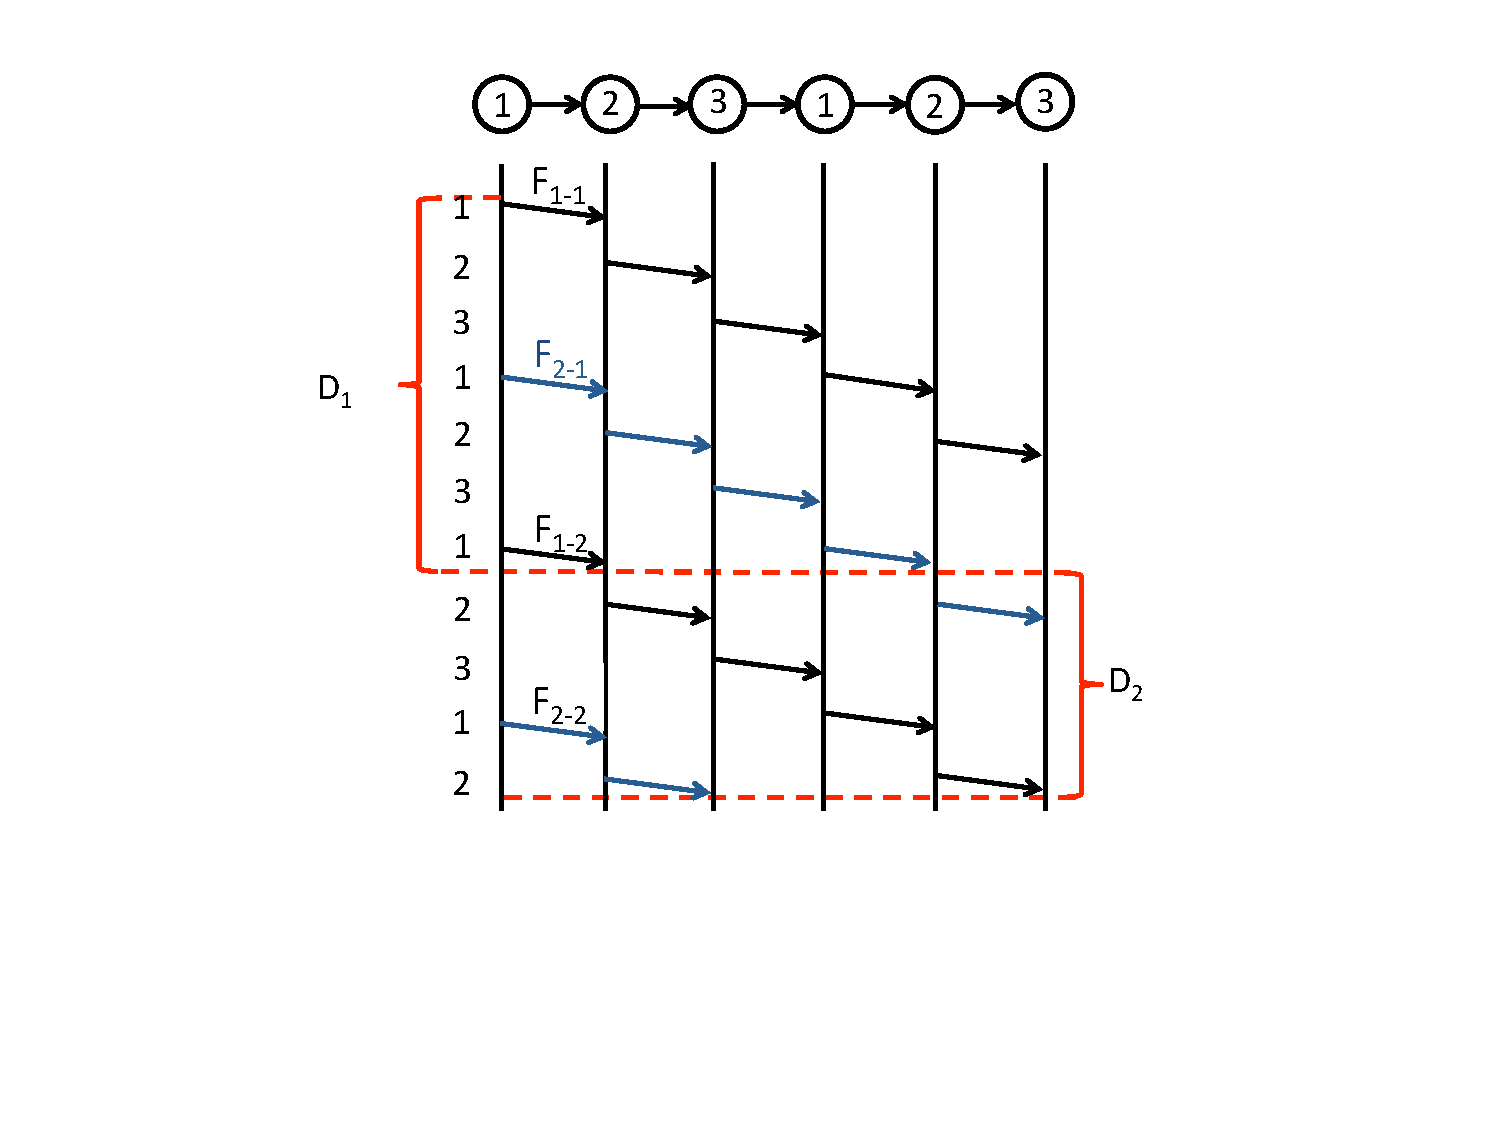
\includegraphics[scale=0.29, clip=true, trim=5mm 0mm 5mm 0mm, valign=t]{figures/delay_limit_expl/delay_expl_fig_a.pdf}
        \label{fig:delay_expl_fig_3}
        }
    \subfigure[$TF = 2$, $CF = 3$, $DF = 2$]{
        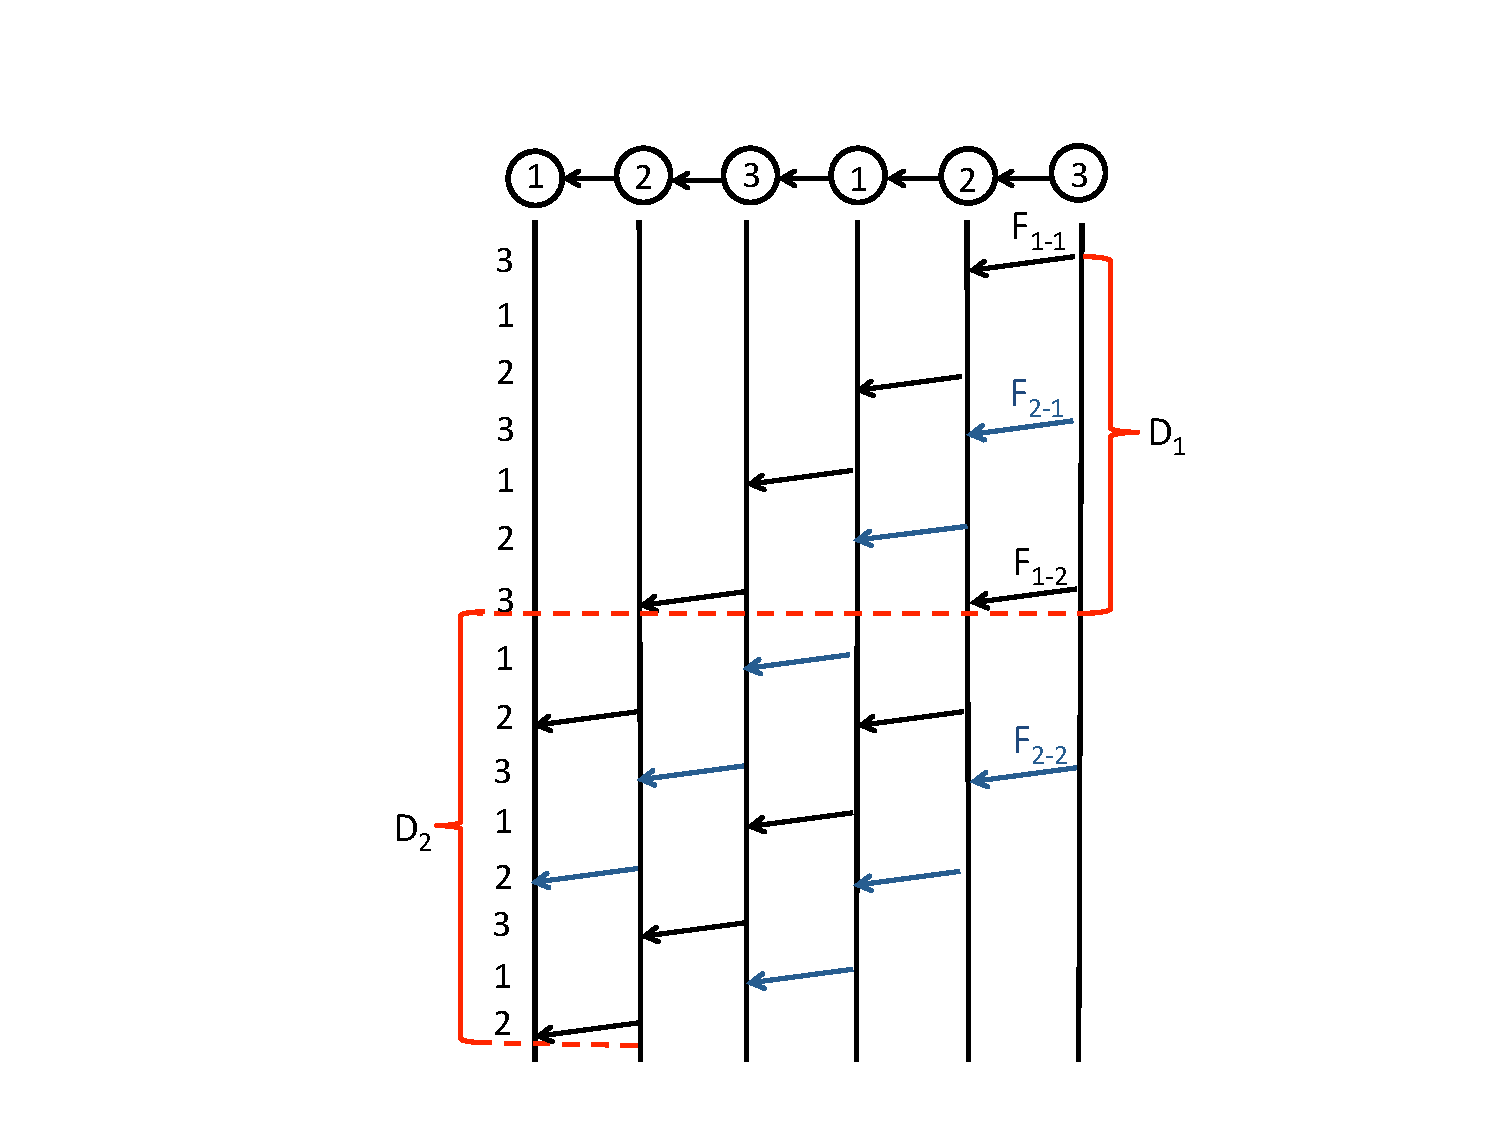
\includegraphics[scale=0.29, valign=t]{figures/delay_limit_expl/delay_expl_fig_b.pdf}
        \label{fig:delay_expl_fig_4}
        }

   \caption{Example of line network using TDMA highlighting source of delays.}
   \label{fig:both_delay_figures}
   \vspace{-5mm}
\end{figure}

Given the nonlinear returns of completeness and importance of timeliness outlined in the previous section, we contend that simply establishing the highest average supportable rate should not be the only goal of a QoI-aware network.  With this knowledge, we set the goal of determining the capacity of a network (and relatedly, the scalability achievable) with respect to {\em QoI requirements}, instead of the maximum throughput.  

\subsection{QoI Satisfiability Framework}
In order to establish the framework, we examine an arbitrary flow, $F_1$, in the network that has a QoI requirement of $\mathbf{q} = \{C, T\}$, where $C$ is the minimum required completeness metric of choice, such as sum similarity as explained above, and $T$ is the required timeliness.  This flow will have a data size requirement, which is given by a chosen QoI function $Q(C)$ like those discussed in Section \ref{sec:qoi_model}.  Using the example applications from \ref{sec:qoi_model}, for example, $Q(C)$ can return the number of images, $k_{req}$, required to achieve the requested completeness $C$ according to established relations like those in Section \ref{sec:qoi_model}.  Assuming each image has an average size of $I_S$, then we can also use $B$ to describe the total number of bits required by the flow, $B=k_{req}*I_S$.  To match realistic network implications, we assume this data will be transmitted in a series of packets with size $P_S$ bits each.  The number of packets per flow, then, is simply $P_N = \lceil B/P_S \rceil$.  We assume that each node in the network can transmit at $W$ bits per second when it is allocated media access.

Our goal is to establish the limits at which this arbitrary flow on average can no longer be completed with the QoI requirements satisfied.  We build and explain our model for achieving this goal by working through an example TDMA line network, a portion of which is shown in Figures \ref{fig:delay_expl_fig_3} and \ref{fig:delay_expl_fig_4} (We discuss addressing non-TDMA networks in Section \ref{sec:discussion}).  In this network, we assume a simple 3-slot TDMA scheme, which allows each node equal time access to the medium and removes any potential interference or hidden terminal issues.  Each node in the figure is labeled with its allocated slot.  For simplicity, we will assume that one slot is appropriately sized to transmit a single packet, i.e., $T_{slot} = P_S/W$ and that packets use static routes calculated beforehand such that the overhead is not a consideration here.

Now, two factors, $D_1$ and $D_2$, contribute to the total delay of completing $F_1$.  The first contributor, $D_1$, is the end to end delay incurred by sending the $B$ bits across the entire path.  To quantify this delay, we must consider several factors beyond just the available bandwidth and number of packets.  First, each node can only utilize its allotted channel time, creating a Channel Factor of $CF = N_{frame}/N_{i}$, where $N_{i}$ is the number of slots allocated to node $i$ and $N_{frame}$ is the total number of slots in each frame.  In this case, $N_{i} = 1, \forall i$ and $N_{frame} = 3$.  The second factor to consider for $D_1$ is the fraction of allocated slots that are utilized by the node to serve flows other than $F_1$ that are either originating in or being routed through nodes on the path of flow $F_1$.  We call the total number of flows competing at node $i$ the Traffic Factor, $TF_i$, of that node.  For any flow, the maximum contributor to delay is the node along the path with the maximum $TF_i$, which we will just call $TF$ here.  Incorporating these considerations into a calculation for $D_1$, we achieve the following expression


\begin{equation}
	D_1 = T_{slot} \cdot P_N \cdot CF \cdot TF
\end{equation}
%\begin{figure}
%\begin{centering}
%    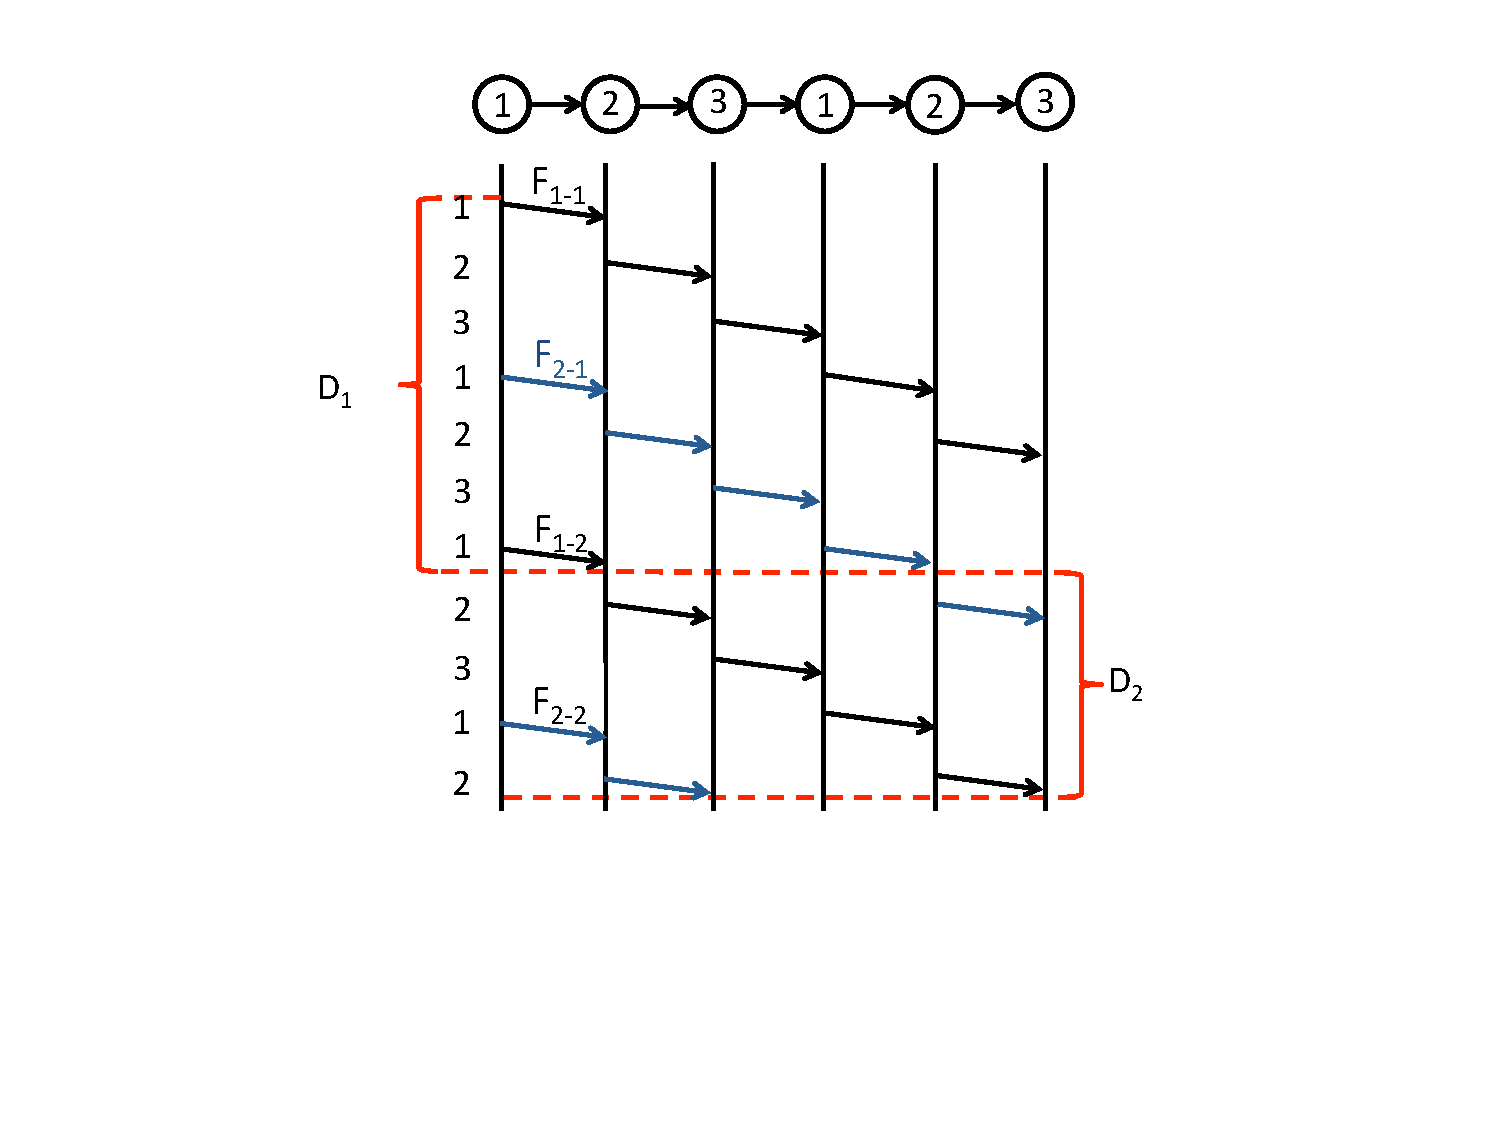
\includegraphics[scale=0.33]{figures/delay_limit_expl/delay_expl_fig_a.pdf}
%    \caption{Example of line network using TDMA highlighting source of delays, $D_1$ and $D_2$.  Here, $TF = 2$, $CF = 3$, and $DF = 1$. }
%    \label{fig:delay_expl_fig_3}
%    \vspace{-3mm}
%\end{centering}
%\end{figure}

Figure \ref{fig:delay_expl_fig_3} depicts the delay of $D_1$ in a simple case of only two flows, $F_1$ and $F_2$, being present, in which case $TF = 2$.  In this example we use flows that consist of only $2$ ($F_{i-j}$ is packet $j$ in flow $i$) packets to portray the delay.  In most real applications, $P_N$ will be much larger, making $D_1$ a good approximation of this delay component.

%\begin{figure}
%\begin{centering}
%    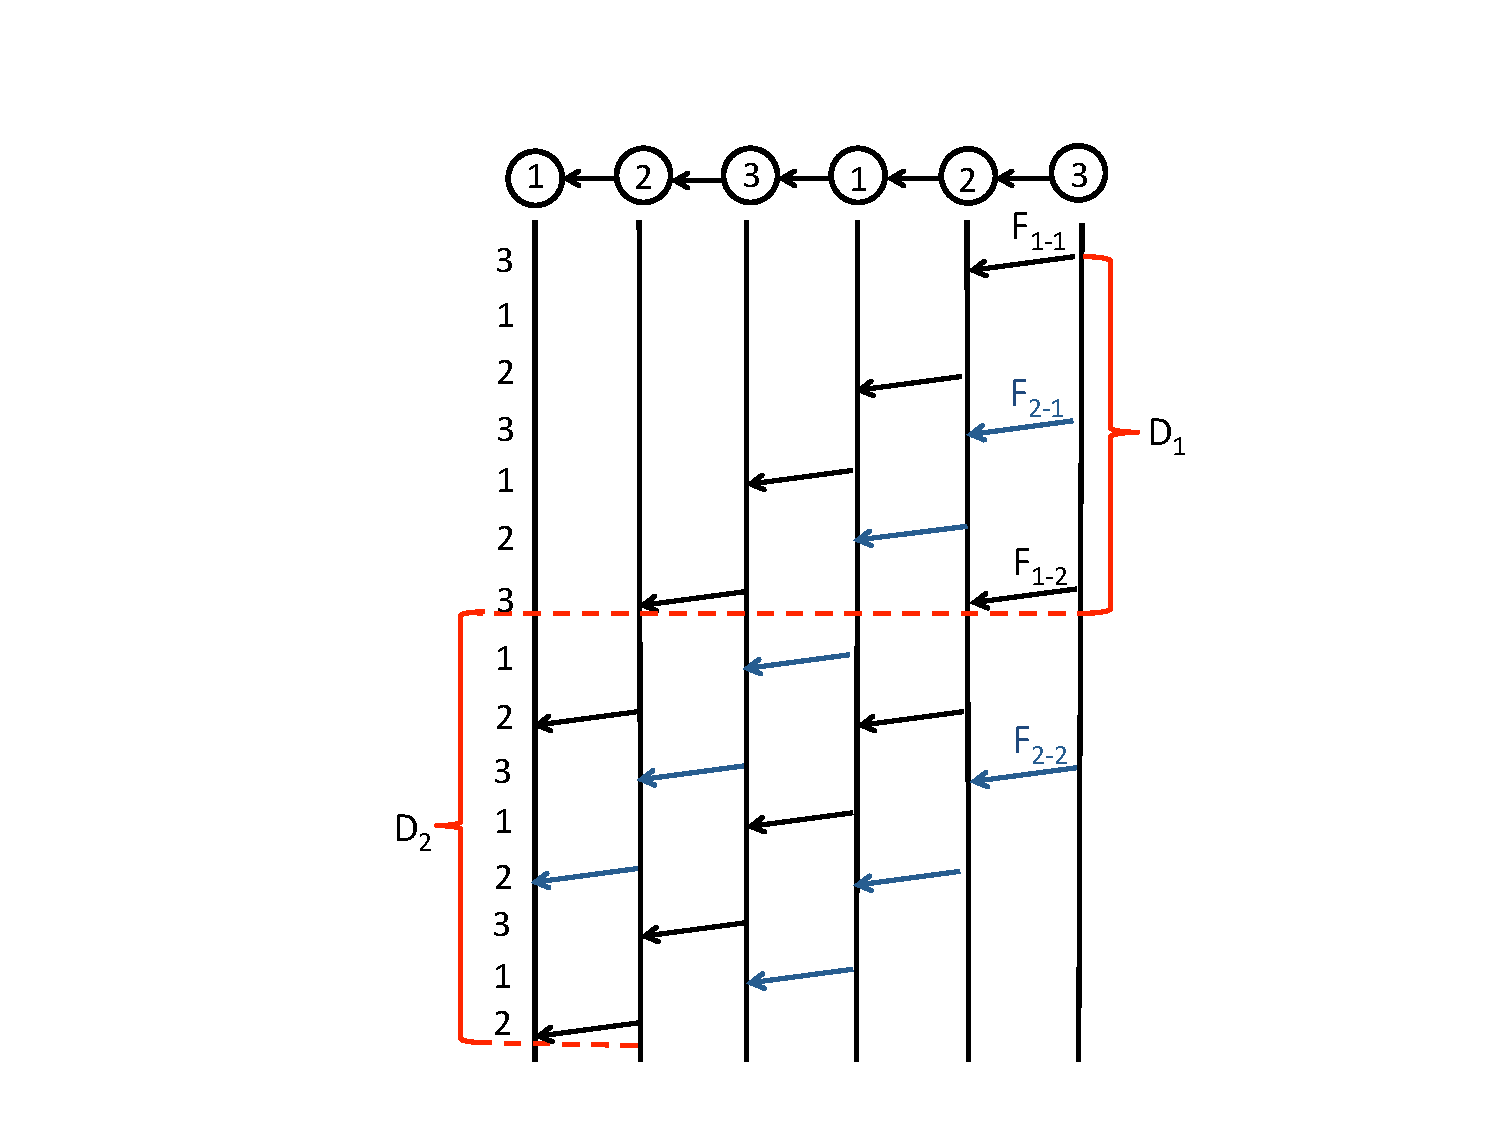
\includegraphics[scale=0.35]{figures/delay_limit_expl/delay_expl_fig_b.pdf}
%    \caption{In the opposite direction, $DF = 2$. ($TF$ and $CF$ are unchanged here.)}
%    \label{fig:delay_expl_fig_4}
%\vspace{-5mm}
%\end{centering}
%\end{figure}

The second delay that exists is due to multi-hop propagation of packets.  This delay is simply the time for a single packet to traverse the path length.  Note that this delay is not necessarily just the path length multiplied by $T_{slot}$, because of possible queuing delays and/or ordering constraints.  We show here how ordering constraints impact this TDMA network.  A node cannot forward a packet from the flow until it receives that packet from the previous hop.  In our line network example, when the direction of the flow matches the nodes' schedule of slots $1-2-3-1-2-3$, as in Figure \ref{fig:delay_expl_fig_3}, each successive node receives a packet on the time slot before it is scheduled, resulting in no extra delay.  For a flow in the opposite direction, though, where nodes are scheduled $3-2-1-3-2-1$, as in Figure \ref{fig:delay_expl_fig_4}, the first slot $1$ is not utilized, because the first node scheduled in time slot $1$ has not yet received a packet in the flow.  Every other slot is wasted, on average, for the initialization of the flow, resulting in approximately twice the delay.  We will use a term that we call the \emph{Delay Factor}, or $DF$, to account for this effect where it exists.

The multi-hop propagation delay, then, is modeled by

\begin{equation}
	D_2 = T_{slot} \cdot DF \cdot (PL - 1)
\end{equation}
where $PL$ is the average path length.

We note several points about this delay factor.  First, in a loaded network, the nodes can and will serve other flows while awaiting the arrival of packets in this flow of focus.  That utilized bandwidth does not, however, preclude this $DF$ impact on delay for the flow of interest, $F_1$.  Any node cannot serve $F_1$ until a packet from that flow has been received.  Second, this delay is only accounted for once per flow because all other packets are pipelined.  All other packets' delay is captured by the end to end delay, $D_1$.  This effect is best illustrated by examining the difference between $D_2$ in Figures \ref{fig:delay_expl_fig_3} and \ref{fig:delay_expl_fig_4}.  Here, we see the multi-hop propagation requires twice the number of slots because every other slot is unused in $F_1$'s propagation.  
%Note that these unused slots may be used by the nodes to transmit packets from a different flow, so the bandwidth may be utilized, but since it cannot be used for flow $F_1$, the delay for this flow is still impacted by $DF$.

To calculate a $DF$ for an entire network, we can calculate a $DF$ for each possible sample path and find the average of these values.  For example, in the case of the line network with a $3$-slot schedule, $DF = 1$ in the direction for Figure \ref{fig:delay_expl_fig_3} and $DF = 2$ in the opposite direction shown in Figure \ref{fig:delay_expl_fig_4}, so the average $DF$ used to approximate average delay in the network is $DF_{line-avg}=1.5$.  

By combining the two components of delay, we can give a relation for a network that will successfully achieve an average flow's data and timeliness requirements:

\vspace{-2mm}
\begin{equation*}
	D_1 + D_2 \leq T 
\end{equation*}
\begin{equation*}
	T_{slot} \cdot P_N \cdot CF \cdot TF + T_{slot} \cdot DF \cdot (PL-1) \leq T
\end{equation*}

Recalling that the time of a slot is determined by the size of a packet, $P_S$, and available channel rate, $W$, in the relation $T_{slot} = P_S/W$, we can substitute to get
\begin{equation*}
	\frac{P_S}{W} \cdot P_N \cdot CF \cdot TF + \frac{P_S}{W} \cdot DF \cdot (PL-1) \leq T
\end{equation*}
Finally, substituting the total number of bits required for a flow $P_S \cdot P_N =  k_{req} \cdot I_S$ (where $k_{req}$ is given by a function of required QoI), and rearranging this inequality, we can obtain a cleaner view of each parameter's impact on network limits:

\vspace{-2mm}
\begin{equation}
	W \cdot T - k_{req} \cdot I_S \cdot CF \cdot TF - P_S \cdot DF \cdot (PL-1) \geq 0	
	\label{eq:general_scal}
\end{equation}

Every network will have its own set of parameters that can be substituted into this general formula, providing a tool to approximate limitations and sensitivity to changes in specific parameters.  To show this usefulness concretely, we provide derived values for a TDMA-based wireless network with several basic topologies.


\begin{figure*}[]
\centering
    \subfigure[Clique Network, $I_S = 9 MB$]{
        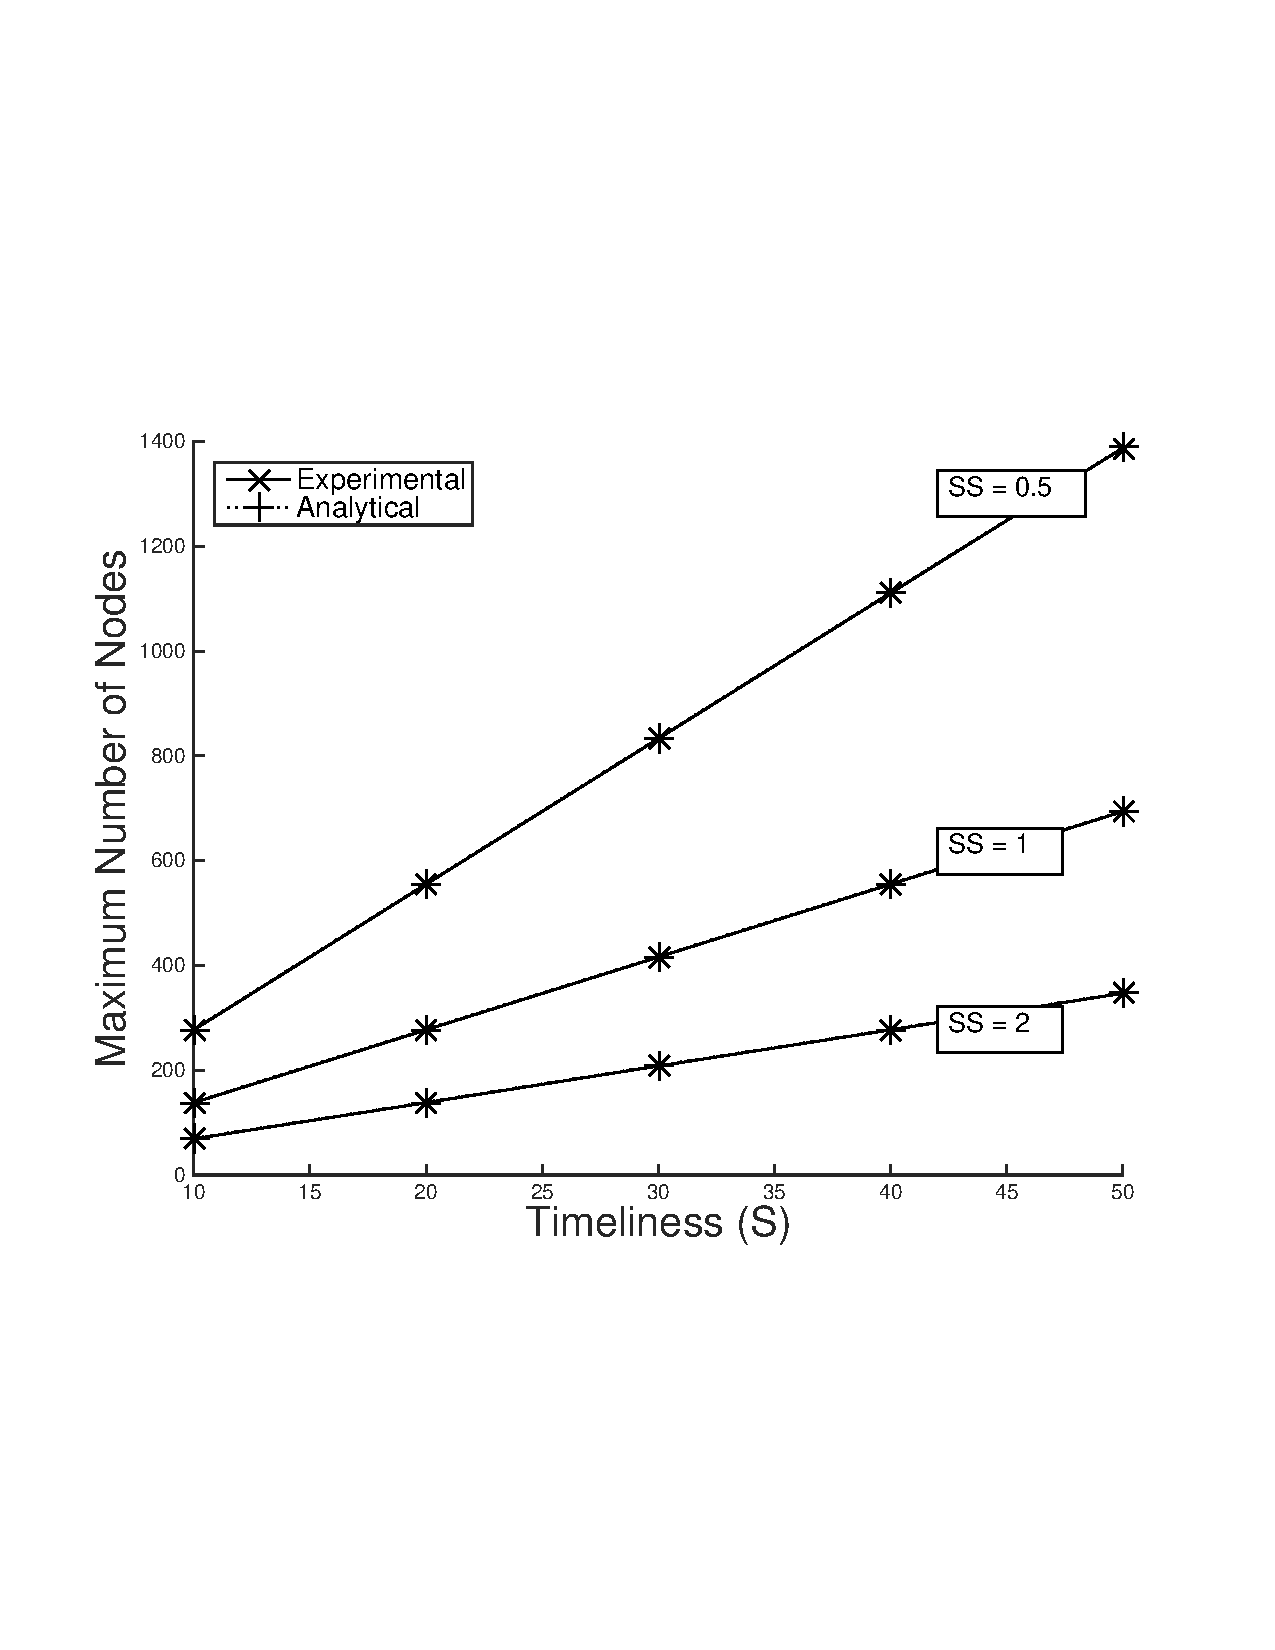
\includegraphics[scale=0.29, clip=true, trim=15mm 65mm 20mm 65mm]{figures/scal_sim_results/clique_uni_2d.pdf}
        \label{fig:scal_vs_qoi_clique}
        }
    \subfigure[Line Network, $I_S = 12 MB$]{
        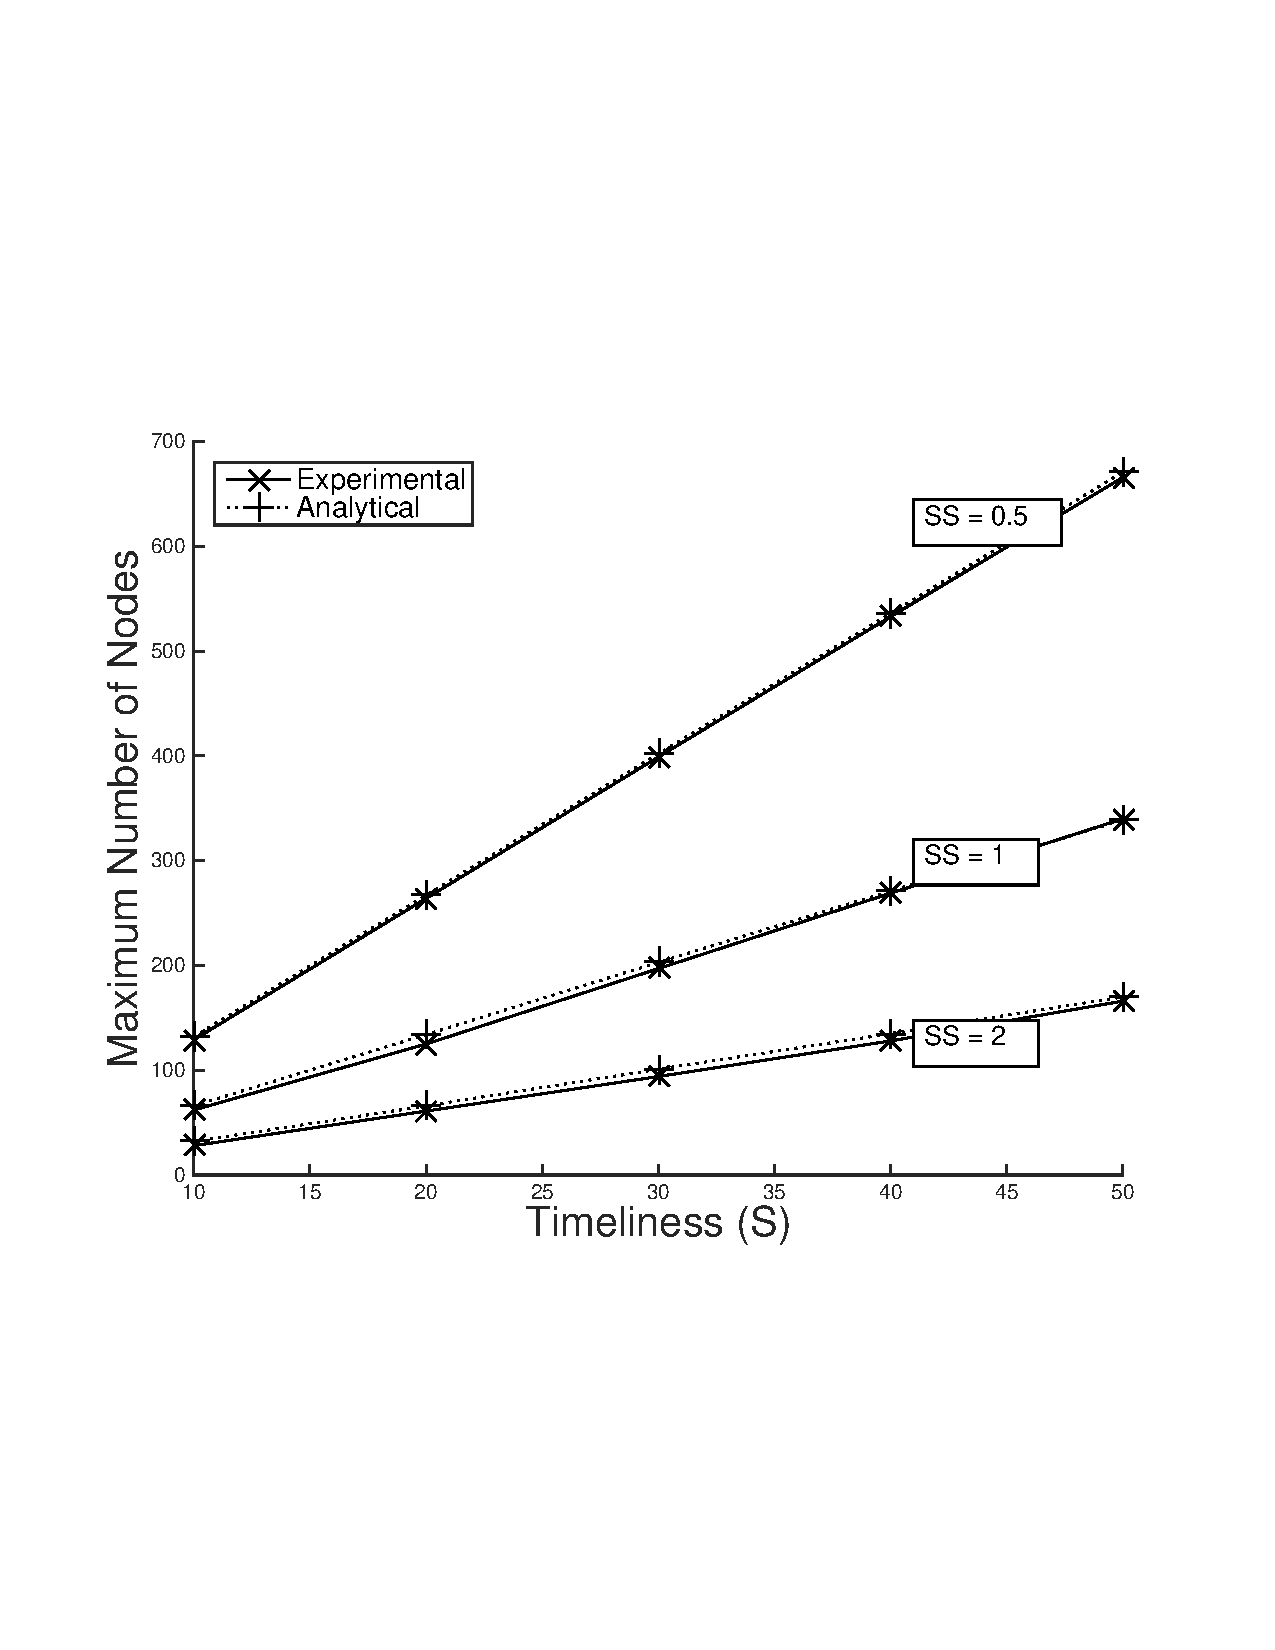
\includegraphics[scale=0.29, clip=true, trim=15mm 65mm 20mm 65mm]{figures/scal_sim_results/line_uni_2d_mhop_2.pdf}
        \label{fig:scal_vs_qoi_line}
        }
    \subfigure[Grid Network, $I_S = 48 MB$]{
        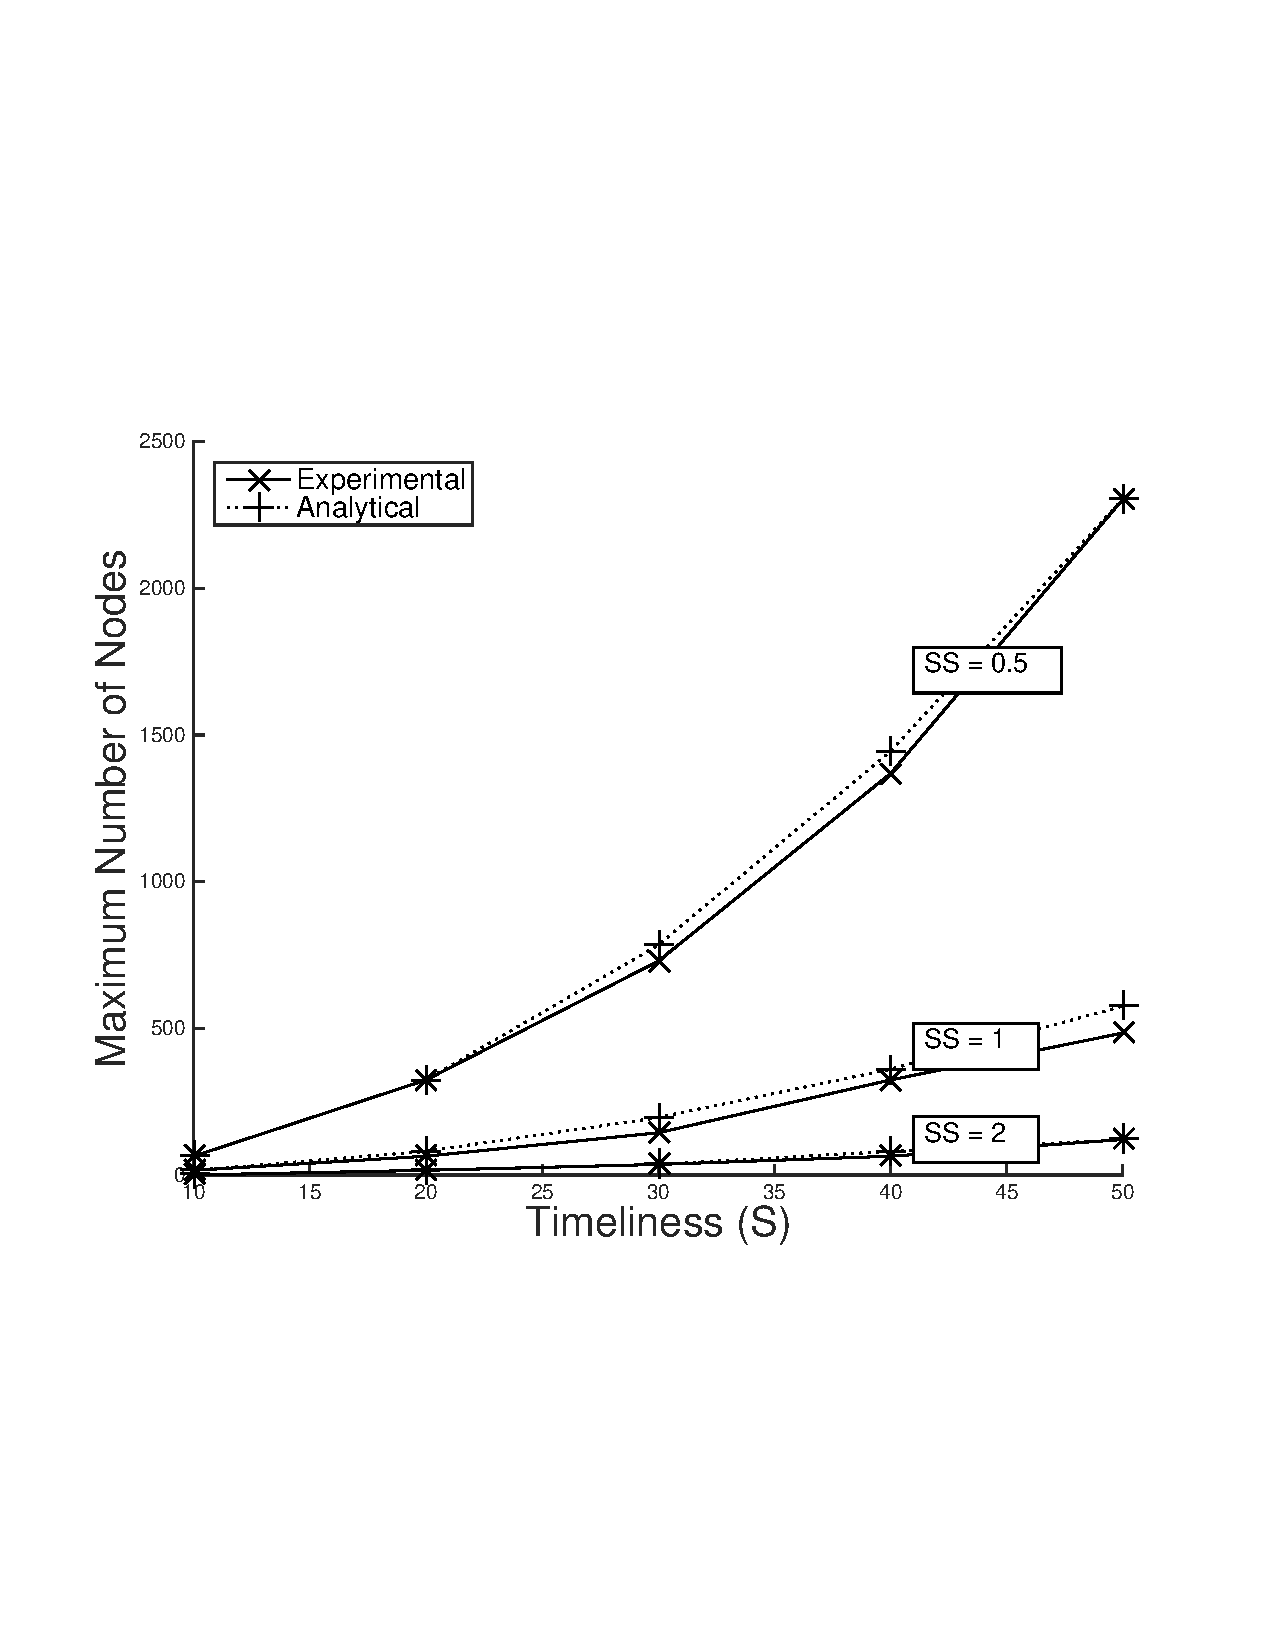
\includegraphics[scale=0.29, clip=true, trim=15mm 65mm 20mm 65mm]{figures/scal_sim_results/grid_uni_2d_mhop_2.pdf}
        \label{fig:scal_vs_qoi_grid}
        }

   \caption{Empirical results match analytical results closely for all performed tests.  Results for each topology and a variety of sum similarity (SS) and timeliness requirements are provided.}
   \label{fig:scal_vs_qoi}

\vspace{-6mm}
\end{figure*}

\subsection{Example of Applying Framework}
\label{sec:example_apply_fw}

We illustrate the application of network signatures to the relationship in (\ref{eq:general_scal}) using an $N$-node TDMA network with three different topologies: clique, line, and grid, also known as a ``Manhattan grid.'' (Discussion of other network control protocols and topologies are addressed in Section \ref{sec:discussion}.)  We adopt a traffic model that uses Top-K queries as an example application.  We assume that all nodes have a set of collected images that are used to respond to Top-K queries.  Each node produces a query with a target image and target QoI, $\mathbf{q} = \{C, T\}$, describing the required completeness (here, we use sum similarity) and timeliness, and sends it to another node chosen at random.  The queried node will respond with the number of images, $k_{req}$, required to achieve the target sum similarity.  Values for $k_{req}$ are taken from the empirical relation in Figure \ref{fig:topkSumSim}\footnote{This application is not necessarily intended to model a known operational scenario, only a generic example to illustrate our model in a simple manner.}.  

\begin{table}[h]
\centering
\begin{tabular}{l|l|l|l|l|}
\cline{2-5}
                            					 & \textbf{CF}  					& \textbf{TF}   				& \textbf{DF}	& \textbf{PL} 			\\ \hline
\multicolumn{1}{|l|}{\textbf{Clique}} 	& N-1 							& 1                              		& 1  			& 1 					\\ \hline
\multicolumn{1}{|l|}{\textbf{Line}}   	& 3   							& $\frac{(N-1)^2}{2(N-2)}$ 	& 1.5 			& $\frac{N}{4}$			\\ \hline
\multicolumn{1}{|l|}{\textbf{Grid}}   	& 5   							& $\sqrt{N}$                       	&  2.5			& $\frac{2}{3} \sqrt{N}$   \\ \hline
\end{tabular}
\caption{CF, TF, DF, and PL values for example topologies}
\label{table:rf_ff_sf_values}
\vspace{-10mm}
\end{table}

Since our goal is to determine the point at which an average flow is no longer sustainable, we derive and use average values for $TF$, $CF$, $DF$, and $PL$ for the network.  In the case of $TF$, we use the value for the node with the largest expected $TF_i$ since flows that are routed through this node are expected to experience that largest delay and are likely to be the first that fail to meet their timeliness requirements.  Values for this example are shown in Table \ref{table:rf_ff_sf_values}, and a derivation of $TF$ for a grid network is included in Appendix \ref{sec:grid_tf_proof}.  Details about deriving the other values are explained in detail in \cite{symptotics_tech_report}.  The following equations can be used to determine QoI and network size limitations, which will be exemplified in the next two sections:

\vspace{3mm}
\noindent
Clique:
\begin{equation}
\label{eq:clique_gen}
	W \cdot T - I_S \cdot k_{req} \cdot (N-1) \geq 0
\end{equation}
Line:
\begin{equation}
\label{eq:line_gen}
	W \cdot T - 3 \cdot I_S \cdot k_{req} \cdot \frac{(N-1)^2}{N-2} - 1.5 \cdot P_S \cdot (\frac{N}{4}-1) \geq 0
\end{equation}
Grid:
\begin{equation}
\label{eq:grid_gen}
	W \cdot T - 5 \cdot I_S \cdot k_{req} \cdot \sqrt{N} - 2.5 \cdot P_S \cdot (\frac{2}{3}\sqrt{N} - 1) \geq 0
\end{equation}


